\documentclass{standalone}
\usepackage{tikz}
\usetikzlibrary{patterns, positioning}

\begin{document}
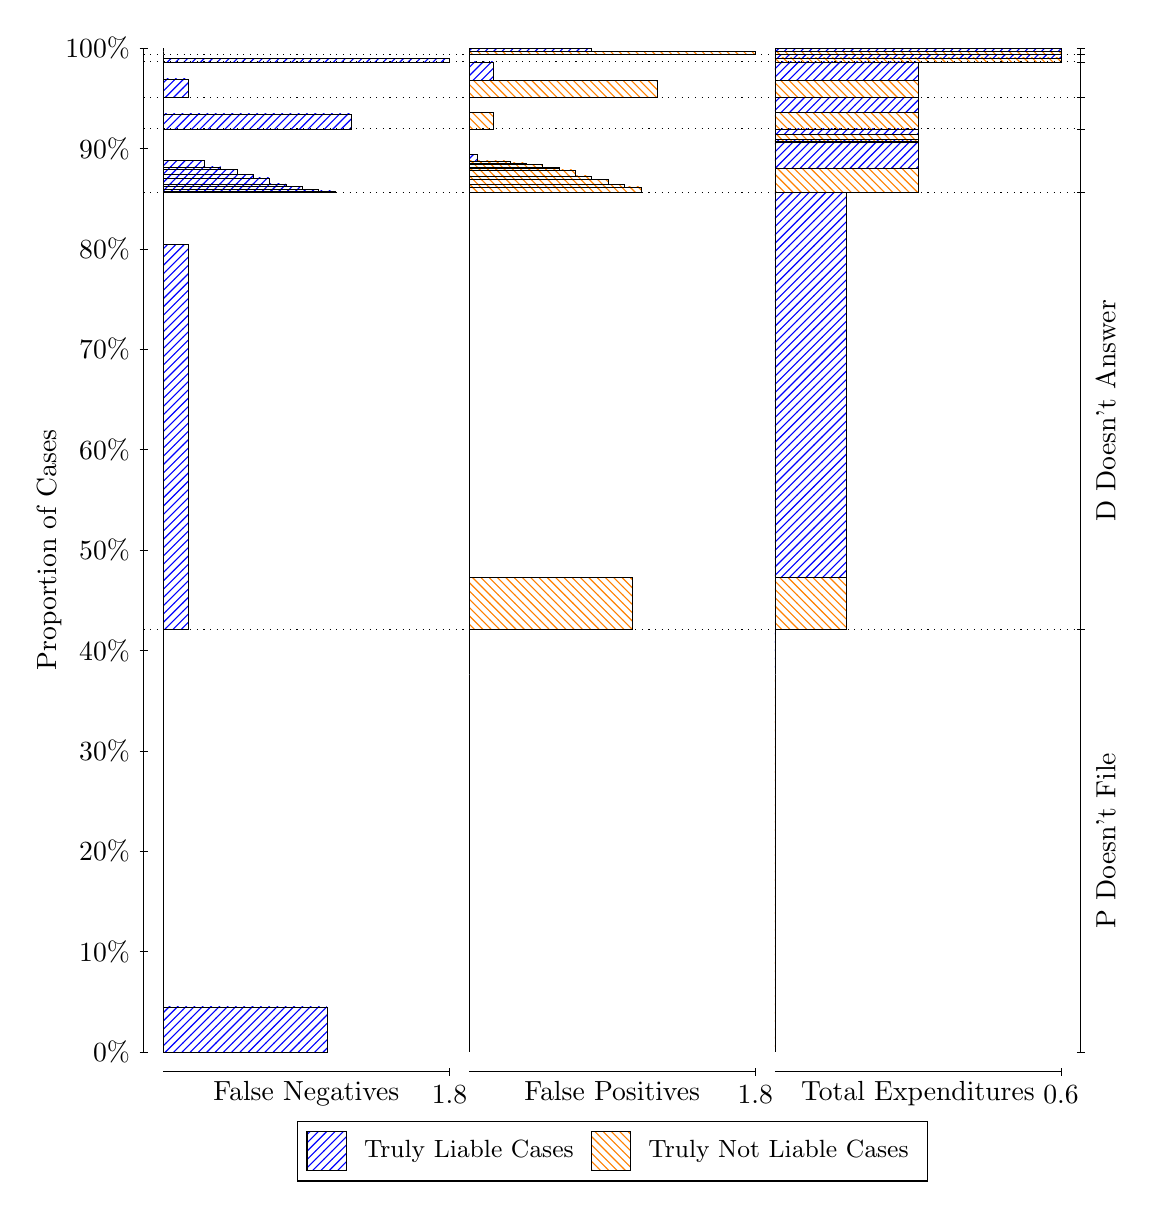
\begin{tikzpicture}
\draw[black, very thin] (1.5,1.75) -- (1.5,14.5);
\node[rotate=90, anchor=center] at (0.3, 8.125) {Proportion of Cases};
\draw[black, very thin] (1.45,1.75) -- (1.55,1.75);
\node[anchor=east] at (1.45, 1.75) {0\%};
\draw[black, very thin] (1.45,3.025) -- (1.55,3.025);
\node[anchor=east] at (1.45, 3.025) {10\%};
\draw[black, very thin] (1.45,4.3) -- (1.55,4.3);
\node[anchor=east] at (1.45, 4.3) {20\%};
\draw[black, very thin] (1.45,5.575) -- (1.55,5.575);
\node[anchor=east] at (1.45, 5.575) {30\%};
\draw[black, very thin] (1.45,6.85) -- (1.55,6.85);
\node[anchor=east] at (1.45, 6.85) {40\%};
\draw[black, very thin] (1.45,8.125) -- (1.55,8.125);
\node[anchor=east] at (1.45, 8.125) {50\%};
\draw[black, very thin] (1.45,9.4) -- (1.55,9.4);
\node[anchor=east] at (1.45, 9.4) {60\%};
\draw[black, very thin] (1.45,10.675) -- (1.55,10.675);
\node[anchor=east] at (1.45, 10.675) {70\%};
\draw[black, very thin] (1.45,11.95) -- (1.55,11.95);
\node[anchor=east] at (1.45, 11.95) {80\%};
\draw[black, very thin] (1.45,13.225) -- (1.55,13.225);
\node[anchor=east] at (1.45, 13.225) {90\%};
\draw[black, very thin] (1.45,14.5) -- (1.55,14.5);
\node[anchor=east] at (1.45, 14.5) {100\%};

\draw[black, very thin] (13.4,1.75) -- (13.4,14.5);
\draw[black, very thin] (13.35,1.75) -- (13.45,1.75);
\node[anchor=west] at (13.35, 1.75) {};
\draw[black, very thin] (13.35,7.1172) -- (13.45,7.1172);
\node[anchor=west] at (13.35, 7.1172) {};
\draw[black, very thin] (13.35,12.664) -- (13.45,12.664);
\node[anchor=west] at (13.35, 12.664) {};
\draw[black, very thin] (13.35,13.473) -- (13.45,13.473);
\node[anchor=west] at (13.35, 13.473) {};
\draw[black, very thin] (13.35,13.876) -- (13.45,13.876);
\node[anchor=west] at (13.35, 13.876) {};
\draw[black, very thin] (13.35,14.324) -- (13.45,14.324);
\node[anchor=west] at (13.35, 14.324) {};
\draw[black, very thin] (13.35,14.415) -- (13.45,14.415);
\node[anchor=west] at (13.35, 14.415) {};
\draw[black, very thin] (13.35,14.5) -- (13.45,14.5);
\node[anchor=west] at (13.35, 14.5) {};

\draw[black, very thin, pattern color=blue, pattern=north east lines] (1.75,1.75) rectangle (3.8262,2.324);
\draw[black, very thin, pattern color=orange, pattern=north west lines] (1.75,2.324) rectangle (1.75,7.1172);
\draw[black, very thin, pattern color=blue, pattern=north east lines] (1.75,7.1172) rectangle (2.0614,12.002);
\draw[black, very thin, pattern color=orange, pattern=north west lines] (1.75,12.002) rectangle (1.75,12.664);
\draw[black, very thin, pattern color=blue, pattern=north east lines] (1.75,12.664) rectangle (3.93,12.686);
\draw[black, very thin, pattern color=blue, pattern=north east lines] (1.75,12.686) rectangle (3.7224,12.7);
\draw[black, very thin, pattern color=blue, pattern=north east lines] (1.75,12.7) rectangle (3.5148,12.739);
\draw[black, very thin, pattern color=blue, pattern=north east lines] (1.75,12.739) rectangle (3.3071,12.775);
\draw[black, very thin, pattern color=blue, pattern=north east lines] (1.75,12.775) rectangle (3.0995,12.85);
\draw[black, very thin, pattern color=blue, pattern=north east lines] (1.75,12.85) rectangle (2.8919,12.897);
\draw[black, very thin, pattern color=blue, pattern=north east lines] (1.75,12.897) rectangle (2.6843,12.957);
\draw[black, very thin, pattern color=blue, pattern=north east lines] (1.75,12.957) rectangle (2.4767,12.99);
\draw[black, very thin, pattern color=blue, pattern=north east lines] (1.75,12.99) rectangle (2.269,13.07);
\draw[black, very thin, pattern color=orange, pattern=north west lines] (1.75,13.07) rectangle (1.75,13.473);
\draw[black, very thin, pattern color=blue, pattern=north east lines] (1.75,13.473) rectangle (4.1376,13.665);
\draw[black, very thin, pattern color=orange, pattern=north west lines] (1.75,13.665) rectangle (1.75,13.876);
\draw[black, very thin, pattern color=blue, pattern=north east lines] (1.75,13.876) rectangle (2.0614,14.109);
\draw[black, very thin, pattern color=orange, pattern=north west lines] (1.75,14.109) rectangle (1.75,14.324);
\draw[black, very thin, pattern color=blue, pattern=north east lines] (1.75,14.324) rectangle (5.3833,14.364);
\draw[black, very thin, pattern color=orange, pattern=north west lines] (1.75,14.364) rectangle (1.75,14.415);
\draw[black, very thin, pattern color=orange, pattern=north west lines] (1.75,14.415) rectangle (1.75,14.454);
\draw[black, very thin, pattern color=blue, pattern=north east lines] (1.75,14.454) rectangle (1.75,14.5);
\draw[black, very thin, pattern color=orange, pattern=north west lines] (5.6333,1.75) rectangle (5.6333,6.5432);
\draw[black, very thin, pattern color=blue, pattern=north east lines] (5.6333,6.5432) rectangle (5.6333,7.1172);
\draw[black, very thin, pattern color=orange, pattern=north west lines] (5.6333,7.1172) rectangle (7.7095,7.7794);
\draw[black, very thin, pattern color=blue, pattern=north east lines] (5.6333,7.7794) rectangle (5.6333,12.664);
\draw[black, very thin, pattern color=orange, pattern=north west lines] (5.6333,12.664) rectangle (7.8133,12.737);
\draw[black, very thin, pattern color=orange, pattern=north west lines] (5.6333,12.737) rectangle (7.6057,12.77);
\draw[black, very thin, pattern color=orange, pattern=north west lines] (5.6333,12.77) rectangle (7.3981,12.83);
\draw[black, very thin, pattern color=orange, pattern=north west lines] (5.6333,12.83) rectangle (7.1905,12.877);
\draw[black, very thin, pattern color=orange, pattern=north west lines] (5.6333,12.877) rectangle (6.9829,12.952);
\draw[black, very thin, pattern color=orange, pattern=north west lines] (5.6333,12.952) rectangle (6.7752,12.977);
\draw[black, very thin, pattern color=orange, pattern=north west lines] (5.6333,12.977) rectangle (6.7752,12.988);
\draw[black, very thin, pattern color=orange, pattern=north west lines] (5.6333,12.988) rectangle (6.5676,13.027);
\draw[black, very thin, pattern color=orange, pattern=north west lines] (5.6333,13.027) rectangle (6.36,13.042);
\draw[black, very thin, pattern color=orange, pattern=north west lines] (5.6333,13.042) rectangle (6.1524,13.067);
\draw[black, very thin, pattern color=blue, pattern=north east lines] (5.6333,13.067) rectangle (5.7371,13.146);
\draw[black, very thin, pattern color=blue, pattern=north east lines] (5.6333,13.146) rectangle (5.6333,13.473);
\draw[black, very thin, pattern color=orange, pattern=north west lines] (5.6333,13.473) rectangle (5.9448,13.684);
\draw[black, very thin, pattern color=blue, pattern=north east lines] (5.6333,13.684) rectangle (5.6333,13.876);
\draw[black, very thin, pattern color=orange, pattern=north west lines] (5.6333,13.876) rectangle (8.021,14.092);
\draw[black, very thin, pattern color=blue, pattern=north east lines] (5.6333,14.092) rectangle (5.9448,14.324);
\draw[black, very thin, pattern color=orange, pattern=north west lines] (5.6333,14.324) rectangle (5.6333,14.375);
\draw[black, very thin, pattern color=blue, pattern=north east lines] (5.6333,14.375) rectangle (5.6333,14.415);
\draw[black, very thin, pattern color=orange, pattern=north west lines] (5.6333,14.415) rectangle (9.2667,14.454);
\draw[black, very thin, pattern color=blue, pattern=north east lines] (5.6333,14.454) rectangle (7.1905,14.5);
\draw[black, very thin, pattern color=orange, pattern=north west lines] (9.5167,1.75) rectangle (9.5167,6.5432);
\draw[black, very thin, pattern color=blue, pattern=north east lines] (9.5167,6.5432) rectangle (9.5167,7.1172);
\draw[black, very thin, pattern color=orange, pattern=north west lines] (9.5167,7.1172) rectangle (10.425,7.7794);
\draw[black, very thin, pattern color=blue, pattern=north east lines] (9.5167,7.7794) rectangle (10.425,12.664);
\draw[black, very thin, pattern color=orange, pattern=north west lines] (9.5167,12.664) rectangle (11.333,12.977);
\draw[black, very thin, pattern color=blue, pattern=north east lines] (9.5167,12.977) rectangle (11.333,13.297);
\draw[black, very thin, pattern color=orange, pattern=north west lines] (9.5167,13.297) rectangle (11.333,13.322);
\draw[black, very thin, pattern color=blue, pattern=north east lines] (9.5167,13.322) rectangle (11.333,13.343);
\draw[black, very thin, pattern color=orange, pattern=north west lines] (9.5167,13.343) rectangle (11.333,13.408);
\draw[black, very thin, pattern color=blue, pattern=north east lines] (9.5167,13.408) rectangle (11.333,13.473);
\draw[black, very thin, pattern color=orange, pattern=north west lines] (9.5167,13.473) rectangle (11.333,13.684);
\draw[black, very thin, pattern color=blue, pattern=north east lines] (9.5167,13.684) rectangle (11.333,13.876);
\draw[black, very thin, pattern color=orange, pattern=north west lines] (9.5167,13.876) rectangle (11.333,14.092);
\draw[black, very thin, pattern color=blue, pattern=north east lines] (9.5167,14.092) rectangle (11.333,14.324);
\draw[black, very thin, pattern color=orange, pattern=north west lines] (9.5167,14.324) rectangle (13.15,14.375);
\draw[black, very thin, pattern color=blue, pattern=north east lines] (9.5167,14.375) rectangle (13.15,14.415);
\draw[black, very thin, pattern color=orange, pattern=north west lines] (9.5167,14.415) rectangle (13.15,14.454);
\draw[black, very thin, pattern color=blue, pattern=north east lines] (9.5167,14.454) rectangle (13.15,14.5);
\draw[black, dotted] (1.5,7.1172) -- (13.4,7.1172);
\draw[black, dotted] (1.5,12.664) -- (13.4,12.664);
\draw[black, dotted] (1.5,13.473) -- (13.4,13.473);
\draw[black, dotted] (1.5,13.876) -- (13.4,13.876);
\draw[black, dotted] (1.5,14.324) -- (13.4,14.324);
\draw[black, dotted] (1.5,14.415) -- (13.4,14.415);
\draw[black, very thin] (1.75,1.5) -- (5.3833,1.5);
\node[anchor=north] at (3.5667, 1.5) {False Negatives};
\draw[black, very thin] (5.3833,1.45) -- (5.3833,1.55);
\node[anchor=north] at (5.3833, 1.45) {1.8};

\draw[black, very thin] (5.6333,1.5) -- (9.2667,1.5);
\node[anchor=north] at (7.45, 1.5) {False Positives};
\draw[black, very thin] (9.2667,1.45) -- (9.2667,1.55);
\node[anchor=north] at (9.2667, 1.45) {1.8};

\draw[black, very thin] (9.5167,1.5) -- (13.15,1.5);
\node[anchor=north] at (11.333, 1.5) {Total Expenditures};
\draw[black, very thin] (13.15,1.45) -- (13.15,1.55);
\node[anchor=north] at (13.15, 1.45) {0.6};

\node[black, centered, rotate=90] at (13.72, 4.4336) {P Doesn't File};
\node[black, centered, rotate=90] at (13.72, 9.8907) {D Doesn't Answer};






\draw (7.449999999999999,1.5) node[draw=none] (baseCoordinate) {};
\begin{scope}[align=center]
        \matrix[scale=0.5, draw=black, below=0.5cm of baseCoordinate, nodes={draw}, column sep=0.1cm]{
            \node[rectangle, draw, minimum width=0.5cm, minimum height=0.5cm, pattern=north east lines, pattern color=blue] {}; &
            \node[draw=none, font=\small] (B) {Truly Liable Cases}; &
            \node[rectangle, draw, minimum width=0.5cm, minimum height=0.5cm, pattern=north west lines, pattern color=orange] {}; &
            \node[draw=none, font=\small] (B) {Truly Not Liable Cases}; \\
            };
\end{scope}

\end{tikzpicture}
\end{document}